\documentclass[12pt,letterpaper]{report}
\usepackage[utf8]{inputenc}
\usepackage[spanish]{babel}
\usepackage{amsmath}
\usepackage{amsfonts}
\usepackage{amssymb}
\usepackage{amsbsy}
\usepackage{graphicx}
\usepackage[left=3cm,right=2.5cm,top=3cm,bottom=2cm]{geometry}
\author{Fernando Manzanares}
\title{Seminario II}
\setlength{\parskip}{4mm}
\usepackage{ragged2e}
\justifying
\usepackage{longtable}
\usepackage{Sweave}
\setlength\parindent{1.25cm}
\usepackage{setspace}
\usepackage{titlesec} 
\usepackage{xcolor}
\titleformat{\chapter}[display]{\bfseries\Huge}{Capítulo \ \Huge\thechapter.}{0.5em}{}
\titlespacing{\chapter}{0pt}{0ex}{1pc}
\usepackage{upgreek}
\widowpenalty=10000  
\clubpenalty=10000
\usepackage{multirow}
\setcounter{secnumdepth}{3} 
\setcounter{tocdepth}{4} 
\usepackage{fancyhdr}
\renewcommand{\labelitemi}{•}
\usepackage{apalike}
\usepackage{cite}
\usepackage{subfigure}
\usepackage{caption}
\captionsetup [table]{name=Tabla}
\captionsetup [figure]{name=Gráfico}


\begin{document}
\Sconcordance{concordance:T_D_SII.tex:T_D_SII.Rnw:%
1 34 1}
\Sconcordance{concordance:T_D_SII.tex:./Portada.Rnw:ofs 35:%
1 28 1}
\Sconcordance{concordance:T_D_SII.tex:T_D_SII.Rnw:ofs 64:%
37}
\Sconcordance{concordance:T_D_SII.tex:./Indice.Rnw:ofs 65:%
1 2 1}
\Sconcordance{concordance:T_D_SII.tex:T_D_SII.Rnw:ofs 68:%
39}
\Sconcordance{concordance:T_D_SII.tex:./Abstract.Rnw:ofs 69:%
1 3 1}
\Sconcordance{concordance:T_D_SII.tex:./Introduccion.Rnw:ofs 73:%
1 20 1}
\Sconcordance{concordance:T_D_SII.tex:./PdelPro.Rnw:ofs 94:%
1 20 1}
\Sconcordance{concordance:T_D_SII.tex:./AbordajeT.Rnw:ofs 115:%
1 3 1}
\Sconcordance{concordance:T_D_SII.tex:T_D_SII.Rnw:ofs 119:%
44 5 1}


\spacing{1.5}

\thispagestyle{empty}

\begin{center}
UNIVERSIDAD DE EL SALVADOR \\ FACULTAD MULTIDISCIPLINARIA DE OCCIDENTE \\ DEPARTAMENTO DE MATEMÁTICAS \\
LICENCIATURA EN ESTADÍSTICA\\
\bigskip

\includegraphics [width=5cm,height=6cm]{Minerva}
\bigskip
\\ ANALISIS DE LA EFICIENCIA ENERGETICA EN LA UNIVERSIDAD DE EL SALVADOR FACULTAD MULTIDISCIPLINARIA DE OCCIDENTE \\
\bigskip
\textbf{MATERIA:}\\ 
SEMINARIO II\\
\textbf{ALUMNO:}\\ 
FERNANDO ERNESTO MANZANARES MORÁN\\
\bigskip
\bigskip
\bigskip
\bigskip
\bigskip
\bigskip

\textbf{SANTA ANA,    DICIEMBRE 2015,   EL SALVADOR}\\
\textbf{CENTRO AMÉRICA}\\


\end{center}


\spacing{1.0}

\tableofcontents 
\thispagestyle{empty}
\spacing{1.5}
\chapter*{Abstract}
\addcontentsline{toc}{chapter}{Abstract}
\pagenumbering{arabic}
Why is conserving energy important? As you can see there are many reasons that conservation is important, ranging from the environment to the economy. The world's dependence on fossil fuels is creating a problem that will affect generations to come. It is important that energy not only be conserved, but also that research continues to find cleaner and better solutions for future generations, in this case the investigation applies a time series to help to UES FMOcc to find a good way to save electrical energy, that means make the energy consumption has to be a priority, in the same line reducing the amount of energy  that they use is a good way to save money, and there are also other benefits to decreasing energy consumption, the efficient use of energy and apply a time series is a priority in this investigation, and this investigation discover that the time series model that describe the energy consumption in UES FMOcc is a SARISMA(0,0,2)*(0,1,1) and the forecasting of this model says that the UES FMOcc has not an efficient energy consumption and have to be fixed.


\textbf{Keywords: Forecast, Time series, energy consumption, conserved energy.}
\chapter*{Introducción}
\addcontentsline{toc}{chapter}{Introducción}

En la actualidad el medio ambiente es uno de los factores más tomados en cuenta con respecto
a la eficiente utilización de los recursos que éste entrega, además de la utilización de técnicas
estadísticas que aporten información para la correcta interpretación de la eficiencia con la que
dichos recursos son utilizados, estas son unas de las razones por la que investigaciones como esta
son necesarios para alcanzar la contribución efectiva en la protección del ambiente, en
términos generales, esta investigacion tiene como objetivo la provisión de 
un diseño favorable en cuanto analsis estadistico, sustentabilidad
ambiental, para alcanzar la eficiencia energética,
normalmente, los aspectos energéticos en cuanto a eficiencia están asociados a la especificación de
las potencias o capacidades de los equipos utilizados en la localización física y geográfica
donde se se encuentran ubicados, y su objetivo principal es alcanzar la utilización máxima de la
capacidad de los aparatos eléctricos con el menor consumo de energía posible, es decir a
través de actividades y tareas como el mantenimiento de sistemas y aparatos eléctricos, por esa
razón se busca la creación de una propuesta para alcanzar dicha eficiencia con el
fin de crear conciencia ambiental en las personas en general, en la UES FMOcc y lograr la
contribución al ambiente a través del ahorro de energía, además de sentar un precedente para
el análisis de datos, que se realizara a través de una serie de tiempo con el objetivo de alcanzar
el preciso análisis de los datos y así tomar la decisiones que generen mayor impacto ambiental.
\chapter{El Problema}
\section{Planteamiento del problema}
Desde hace ya varios años, la protección al medio ambiente se ha ido convirtiendo en un tema de mucha importancia,
tanto así, que varios países del mundo han comenzado a adoptar políticas para la conservación de este, dichas politicas van desde, el tratamiento desechos solidos hasta el ahorro de energía y cada día que pasa se adoptan muchas mas; entonces la NO protección del ambiente esta generando dichas reacciones en las poblaciones de todos los países alrededor del mundo, ya que en la actualidad se viven problemas como la contaminación y escasez de agua, contaminación del aire, degradación de los suelos y descenso de la productividad agrícola, deforestación, residuos sólidos y peligrosos, pérdida de la diversidad biológica, desgaste de la capa de ozono y cambios climáticos,todos estos problemas afectan a los países, de manera desigual, según el grado de su desarrollo, de su estructura económica y de las políticas ambientales que aplican, es decir para combatir el deterioro ambiental se llevan a cabo dos tipos de políticas; las que procuran relacionar el desarrollo con el medio ambiente a nivel general de población, recursos, legislación y tecnologías, y las que se orientan a problemas específicos, uno de los factores mas importantes al interior de estas problemáticas es el ahorro de energía, este factor entra en el segundo tipo de política anteriormente mencionada, es por eso que paises desarrollados están comenzando a implementar medidas que buscan dicho ahorro y ademas buscan consumir energía pero de manera eficiente.

En El Salvador, el problema de la eficiencia enérgetica no ha sido abordado desde el punto de vista estadistico, es decir, la aplicación de tecnicas estadisticas para investigar dicho problema,
normalmente, los aspectos energéticos en cuanto a eficiencia están asociados a la especificación de
las potencias o capacidades de los equipos utilizados en la localización física y geográfica
donde se se encuentran ubicados, y su objetivo principal es alcanzar la utilización máxima de la
capacidad de los aparatos eléctricos con el menor consumo de energía posible, por esa razon esta investigación busca la implementación de una serie temporal para el analisis de los datos del consumo electrico mensual en la Universidad de El Salvador Facultad Multidisciplinaria de Occidente (UES FMOcc), además, desarrollar proyeciones apartir de dicho modelo para analizar e interpretar el comportamiento del consumo eléctrico y sentar un presedente a nivel academico y teórico sobre el abordaje que se le pueden dar a este tipo de problemas, a estose agrega, contribuir en la protección del ambiente y generar conciencia para cambiar los habitos del consumo electrico, en la misma linea tambien pretende responder a las siguientes preguntas ¿Será eficiente el consumo eléctrico en la UES FMOcc? ¿Es posible alcanzar la eficiencia enérgetica en los edificios y aulas de la UES FMOcc? ¿Está el consumo energetico en la UES FMOcc creciendo a través del tiempo? ¿Cuáles son los periodos de tiempo donde se consume mas energia eléctrica? ¿Cuánta energía podria ahorrase si se lograra la eficiencia enérgetica?

\newpage
\section{Justificación}
Esta investigación pretende analizar y desarrollar proyeciones sobre los datos del consumo electrico en la UES FMOcc, para descubrir si existe o no eficiencia energetica además de la aplicación de un modelo estadistico autoregresivo integrado de media movil para datos estacionales y de esta manera poder interpretar los datos del consumo energetico de manera nueva y mas precisa, la importancia de realizar esta investigación se basa principlamente en el aporte teórico nuevo que sentara una base para el desarrollo de futuras investigaciones de esta índole, además de la aplicacion de tecnicas propiamente estadisticas para el monitoreo del comportamiento del consumo enérgetico en la UES FMOcc, esto con el fin de identificar los espacios de de tiempo donde se consume la mayor cantidad de energía eléctrica y de esta manera poder abordar de manera efectiva la problemática de eficiencia enérgetica, a esto se agrega que esta investigación tracenderá en el tiempo y será util durante los proximos 18 meses apartir de agosto de 2015 debido al tipo de tecnica utilizada para desarrollar las proyeciones y por último la contribución a la protección del ambiente una vez alcanzada la eficiencia en los sistemas electricos de la UES FMOcc, en el aspecto económico la realización de esta investigación resultaria favorable ya que la eficiencia enérgetica ademas de contribuir al ambiente sugiere una reducción en los costos del consumo enérgetico. 


\newpage
\section{Objetivos de la investigación}
\subsection{Objetivo general}

\begin{itemize}
\item Analizar los datos del consumo eléctrico a través de la utilización de una serie
temporal, para la interpretación de el comportamiento del consumo enérgetico a través del tiempo y si existe eficiencia energética en la UES FMOcc en los próximos 18 meses.
\end{itemize}

\subsection{Objetivos específicos}

\begin{itemize}
\item Desarrollar y analizar las proyecciones de los datos del consumo eléctrico de la
FMOcc a través de modelos estadísticos de series temporales para los próximos 18
meses.

\item Identificar el periodo de tiempo donde el consumo energetico es mas bajo y analogamente donde es mas alto.

\item Conecer la cantidad de energia y costos que podrían reducirse para contribuir al ambiente si se lograra la eficiencia energetica.  

\end{itemize}

\newpage
\section{Hipótesis}
\textbf{ Hipotesis 1.} 

$H_0$ No existe eficiencia energetica en los edificios de la Universidad de El Salvador Facultad Multidisciplinaria de Occidente.

$H_1$ Existe eficiencia energetica en los edificios de la Universidad de El Salvador Facultad Multidisciplinaria de Occidente.

\textbf{ Hipotesis 2.}

$H_0$ El consumo energetico en la Universidad de El Salvador Facultad Multidisciplinaria de Occidente es creciente a través del tiempo.

$H_1$ El consumo energetico en la Universidad de El Salvador Facultad Multidisciplinaria de Occidente no es creciente a través del tiempo.


\textbf{ Hipotesis 3.}

$H_0$ Los periodos donde más energia electrica se consume son durante los ciclos academicos desarrollados en la Universidad de El Salvador Facultad Multidisciplinaria de Occidente. 

$H_1$ Los periodos donde más energia electrica se consume no son durante los ciclos academicos desarrollados en la Universidad de El Salvador Facultad Multidisciplinaria de Occidente.





\chapter{Fundamentación teórica}
\section{Antecedentes}

  \subsection{Eficiencia Energetica en España}

Las variaciones marginales del consumo de energía en España, que son
debidas tanto a la evolución de la actividad económica como a las
modificaciones de la intensidad energética, implican variaciones equivalentes
en las importaciones de petróleo, es decir españa depende mucho del petroleo como fuente de energía, en la estrategia de Ahorro y Eficiencia Energética que España posee se ha previsto una mejora
sostenida de la intensidad energética durante los próximos años. Pero lo
realmente importante a señalar no son las cifras absolutas de mejora, sino el
porcentaje de mejora de la eficiencia que en la práctica se puede conseguir, es decir la conciencia ambiental juega un papel fundamental para un pais como España. 

 \subsection{Eficiencia Energetica en Chile}
 
¿Cómo es el consumo energético en Chile?

El grupo de energéticos que más se consume corresponde a los derivados del petróleo, que representa el 54\% del consumo final secundario, prácticamente la totalidad de los derivados debe ser importada o son producto de la refinación de petróleo crudo, cuya importación alcanza al 96,5\%,el segundo energético más utilizado es la electricidad, que representa el 19,2\% del consumo final; le sigue la leña con el 17,8\%, el gas natural con el 5,5\%, esto según el estudio de mercado en chile, en febrero de 2012 se dio a conocer la Estrategia Nacional de Energía 2012-2030, que se basa en 6 pilares fundamentales entre ellos el aborade de la Eficiencia energetica. 


 \subsection{Eficiencia Energetica en México}
 
 Históricamente, el sector energético de México ha dependido de los hidrocarburos para satisfacer la energía que demanda el país. Sin embargo, la producción nacional de energía primaria ha disminuido constantemente desde 2004, debido a la caída inercial que presentó la producción de petróleo, que se originó principalmente por la declinación del yacimiento de Cantarell. Por otro lado, el consumo nacional de energía se ha mantenido a la alza por varios años,
lo anterior ha llevado a reflexionar sobre el riesgo que enfrenta la productividad del país ante una tendencia que haga vulnerable la eficiencia energética en los siguientes años, hoy en día una preocupación prioritaria de los gobiernos modernos en todo el mundo se focaliza en promover el aprovechamiento sustentable del uso de la energía y la utilización de nuevas fuentes de energía, sin menoscabar aspectos claves que propicien el crecimiento económico, la seguridad energética y la adaptación al cambio climático de cada país, dada la situación actual, el Gobierno de la República atiende la necesidad de llevar a cabo acciones para el aprovechamiento sustentable de la energía que contribuyan a la seguridad energética y económica del país, promoviendo la eficiencia energética en los diversos sectores productivos y de consumo de energía en México, a partir del reconocimiento de las áreas de oportunidad y sus fortalezas institucionales\cite{Mexico}.

\subsection{Eficiencia Energetica en El Salvador}

Hablar de ahorro energético es complejo, siendo la energía un elemento básico para la productividad, por lo que al buscar una solución viable y sostenible la propuesta es lograr un uso eficiente de este recurso. los programas de eficiencia energética deben involucrar al estado, al sector empresarial y a la sociedad civil, y establecer como ejes principales la generación de una cultura de uso racional de la energía en la población, la formulación de políticas nacionales y el diseño de un marco regulatorio adecuado, que permitan el correcto balance entre el crecimiento económico y la demanda en el consumo eléctrico, acompañar el crecimiento económico del país, suministrando el servicio eléctrico requerido por hogares, comercios e industrias; bajo un enfoque sostenible que permite asegurar la protección de los recursos naturales para las generaciones futuras, El Salvador cree que la sostenibilidad tiene entre uno de sus principales fundamentos la eficiencia energética, por ello se ocupa de brindar de forma permanente capacitación, información y asesoría, fortalecer sus herramientas tecnológicas para asistir a sus clientes, y disponer de programas permanentes dirigidos a crear una cultura de uso responsable y seguro de la energía eléctrica en las nuevas generaciones, hay propuestas, pero no estan siendo llevadas a cabo.\cite{MIESA}

\section{Teorías acerca de la eficiencia enérgetica}

Aunque a priori pudiera pensarse que “eficiencia energética” es un concepto
autoexplicativo y que,el alcance del mismo está claramente
delimitado, la realidad muestra que se trata de un término dificil, como lo
demuestran las dificultades que encuentran algunos expertos para ponerse de
acuerdo a la hora de establecer indicadores específicos de eficiencia
energética, en el caso de esta investigacion se abordara de manera mas sencilla, basandose unicamente en la cantidad de energía consumida y si esta se puede reducir, dejando claro el hecho de que si se puede encontrar una manera de reducir el consumo energetico entonces puede lograrse la eficiencia energetica.

A manera de ejemplo puede suponerse, la maroria reconoce como
medida de eficiencia energética el aislamiento de las viviendas, al mantener el
nivel de confort con un ahorro de energía (en el caso de la UES FMOcc la maximizacion de las capacidades de los aparatos electricos con el consumo minimo de energía), pero este ahorro energético que se
produce a nivel individual no necesariamente se visualiza a nivel del conjunto
de la comunidad, un incremento en el número de viviendas construidas o un
aumento de la demanda de confort (más electrodomésticos, aire
acondicionado, etc.), pueden enmascarar las mejoras en la eficiencia
energética alcanzadas a nivel individual, es decir puede que no se logre la eficiencia energetica deseada. 

\section{Teorías estadísticas}

  \subsection{Estacionariedad, Estacionalidad y transformaciones}

Los datos en los negocios, ingeniería, medicina y en otras áreas de investigación científica generalmente se recolectan en forma de series temporales, es decir, son recolectados de manera secuencial en un lapso determinado de tiempo que generalmente describen el comportamiento de una o varias variables que son observadas, de manera específica el objetivo principal que persigue una serie temporal es: entender e interpretar la dinámica de estructuras dependientes que forman las observaciones en el tiempo consigo mismas (de una variable, que se retroalimenta) o el efecto que pueden tener las relaciones de este tipo de estructuras temporales con otras (varias variables); los beneficios que puede lograr el claro entendimiento de este tipo de estructuras temporales son principalmente las predicciones precisas de las observaciones en el futuro en una variedad de esquemas de información en este caso el del consumo energético.

"Formalmente una serie de tiempo se define como un conjunto de observaciones repetidas de la misma variable tal como:$ Y_1, Y_2, · · · , Y_T$. A partir de esta caracterización se desprenden dos conceptos fundamentales en el análisis de series de tiempo. Los mismos se definen mediante la imposición de algunos supuestos
sobre el comportamiento de $Y_t$". \cite{Isaac}

Uno de estos supuestos es la estacionariedad de una variable observada en el tiempo ($Y_t$); de manera teórica, esto equivale a decir que las observaciones están fluctuando en torno a un mismo valor, es decir dichas observaciones poseen media constante, además para complementar este concepto es necesario tomar en cuenta que los datos observados deben estar fluctuando de manera similar en un lapso de tiempo, en otras palabras deben poseer varianza constante, a esto se agrega que la covarianza entre dos observaciones dependa únicamente de su separación y no del instante en el tiempo en el que se toman, en la misma línea cabe destacar que en la práctica, la mayoría de las series que se analizan poseen ausencia de estacionariedad, es decir, no poseen media ni varianza constante y que la covarianza depende del instante del tiempo y no de su separación  (son no estacionarias), de manera formal es posible definir que para el análisis de una serie temporal, la estacionariedad, es estrictamente necesaria, ya que si una serie cumple esta condición esta será invariante en el tiempo (en teoría), esta es una de las condiciones más fuertes que debe cumplir una serie en el tiempo.

El autor \cite{Tsay}, define de manera formal la estacionariedad (debil) de una serie de tiempo si se cumple:

\begin{enumerate}
\item $E(Y_t) = \mu$
\item $Cov(Y_t,Y_{t-\ell}) = Y_\ell$, y solo depende de $\ell$.
\end{enumerate}

Otro concepto importante es el de la estacionalidad, esto quiere decir que la serie temporal presenta un comportamiento cíclico, es decir dicho ciclo puede repetirse semanal,  mensual, trimestral, semestral e incluso anualmente, todo depende del tipo de variable que se esté observando, cuando esta característica está presente la serie adopta el nombre de serie de tiempo estacional, para el análisis de este tipo de series es necesario aplicar ciertos procedimientos para lograr un ajuste estacional (remover la estacionalidad) y luego conseguir que esta nueva serie cumpla la condición de ser estacionaria; para saber si una serie es estacional, se utiliza el correlograma comúnmente denominado grafico de auto correlaciones simples, donde se observan los retardos con mayor correlación durante un lapso determinado de tiempo esto con el fin de encontrar cierta repetitividad en cada periodo observado, posteriormente una vez detectada la estacionalidad pueden utilizarse técnicas como la diferenciación estacional definida por, $\triangle_s Y_t = y_{t}-y_{t-s}$; de una serie estacional $Y_t$ con periodicidad "s", cabe mencionar que esta expresión es similar a la diferenciación para una serie no estacional $Y_t$, definida por $Y_t=y_{t}-y_{t-1}$; \cite{Tsay}

Una vez detectada la estacionalidad o la no estacionalidad de la serie, es necesario que la serie sea estacionaria, para lograr esto, se utiliza comúnmente la técnica de diferenciación no estacional y la diferenciación estacional, esta última solo si la serie es estacional, este proceso se lleva a cabo para lograr que la serie sea constante en media; para conseguir varianza constante comúnmente se utilizan transformaciones de escala como la logarítmica o se usa la transformacion de box-cox para tomar la mejor decisión, dicha transformacion esta definida por:

\begin{center}
$f(x) = \left\{
\begin{matrix}
  \dfrac{x^\lambda - 1}{\lambda}   &  \mbox{para } \lambda \not= 0 \\
    log(x)                        &   \mbox{para } \lambda = 0 
\end{matrix}\right.$
\end{center}

Esta transformación consiste en calcular un valor de lambda y aplicar la transformación, cabe mencionar que si $\lambda$ se aproxima a cero la transformacion equivale a el $log(x)$ si $\lambda$ es igaual a $\frac{1}{2}$ la tranasformación equivale a la raiz cuadrada y si $\lambda$ es igual a $-1$ enconces multiplicar por el reciproco de cada dato sería su equivalente, algunos programas estadísticos facilitan el calculo de $\lambda$ a partir de los datos en esta investigación se utilizara el programa R.\cite{Cryer}

Ahora necesario probar estadisticamente si la serie es estacionaria, para eso se utiliza la prueba de Dickey Fuller (DF) que contrasta la hipótesis nula de que una serie es no estacionaria si el polinomio asociado a esta posee raíz unitaria, la decisión sobre este contraste se toma a partir del valor asintótico (P-valor) arrojado por la prueba, si este es menor a la significancia utilizada entonces se rechaza la hipótesis nula y puede concluirse que la serie es estacionaria, por último es importante mencionar que “el test DF, es poco potente, corremos por tanto el riesgo de admitir la presencia de una raíz unitaria cuando en realidad no existe” \cite{Ramon}. En la misma línea debe saberse por que tomar la decisión de utilizar una prueba como la de DF para probar estacionariedad, se sabe que una variable simple auto regresiva tiene la forma $x_t=\alpha x_{t-1}+\varepsilon_t$; \cite{Daniel2001}, si se sustrae $x_{t-1}$ de ambos lados el resultado es $\triangle x_t=(\alpha-1) x_{t-1}+\varepsilon_t$; esta ecuación es la base de la prueba DF, “el estadístico de prueba es el estadístico t sobre la variable rezagada. Si $\alpha>1$ el coeficiente de la variable rezagada será positivo, si "$\alpha$" es igual a la unidad $(\alpha-1)$ será igual a cero. En ambos casos $x_t$ será no estacionaria” \cite{Commandeur2007}.

\subsection{Función de autocorrelacion simple (FAS o ACF)}

Cuando se mide una variable a lo largo del tiempo, las observaciones en
diferentes periodos a menudo están relacionadas o correlacionadas. Esta correlación se mide usando el coeficiente de autocorrelación. La autocorrelación
es la correlación que existe entre una variable retrasada uno o más períodos
consigo misma.
Los patrones de datos que incluyen componentes como tendencia y estacionalidad pueden estudiarse usando autocorrelaciones. Los patrones se identifican
examinando los coeficientes de autocorrelación de una variable en diferentes
retrasos de tiempo.

La ecuación siguiente ecuacion es la fórmula para calcular el coeficiente de autocorrelación $r_k$
entre las observaciones $Y_t$ y $Y_{t-k}$, que se encuentran a k periodos de distancia.

\begin{center}
$\rho_k = \dfrac 
{\sum_{t=k+1}^{n} (Y_t-\bar{Y})(Y_{t-k}-\bar{Y})}
{\sum_{t=1}^{n} (Y_t - \bar{Y})^2}; \mbox{ Para } k = 1,2,3,...$
\end{center}

Donde,

\textbf{$\rho_k$}: Es el coeficiente de autocorrelación para un retraso de k periodos.

\textbf{$\bar{Y}$}:Es la media de los valores de la serie de tiempo.

\textbf{$Y_t$}:Es la observación en el periodo t.

\textbf{$Y_{t-k}$}:  Es la observación k periodos anteriores o durante un periodo t - k.

\subsection{Función de autocorrelacion parcial (FAP o PACF)}

La autocorrelacióon parcial mide la correlación entre dos variables separadas por k periodos cuando no se considera la dependencia creada por los retardos intermedios existentes entre ambas, Los coeficientes de autocorrelaci´on para diferentes retrasos de tiempo de una
variable pueden usarse para contestar las siguientes preguntas acerca de una
serie de tiempo:

\begin{enumerate}
\item  Los datos son ruido blanco.\footnote{El proceso t se define como ruido blanco si cumple con
las siguientes condiciones:\\
1. La esperanza de $Y_t$ o promedio es igual a 0 para todos los periodos t. Esto es $E(Y_t) = 0$ para toda t.\\
2. La varianza de $Y_t$ es constante y por consiguiente independiente del tiempo. Esto es $var(Y_t) = \sigma^2$.}
\item  Los datos muestran una tendencia (son no estacionarios).
\item  Los datos son estacionarios.
\item  Los datos son estacionales.
\end{enumerate}

Si una serie es aleatoria, las autocorrelaciones entre $Y_t$ y $Y_{t-k}$ para cualquier
retraso de tiempo k son cercanas a cero. Los valores sucesivos de una serie
de tiempo no est´an relacionados entre sí. "Si una serie muestra una tendencia,
las observaciones sucesivas están altamente correlacionadas y es típico que
los coeficientes de correlación sean significativamente diferentes de cero, para
los primeros retrasos de tiempo, y de forma gradual tienden a cero conforme
se incrementa el número de retrasos" \cite{Isaac}.

Para identificar si una autocorrelacion es significativamente diferente de cero se utiliza el correlograma, y apartir de este se toma la decisión sobre los retardos, por ejemplo:

\begin{figure}[htb]

\centering
\caption{Correlograma} 
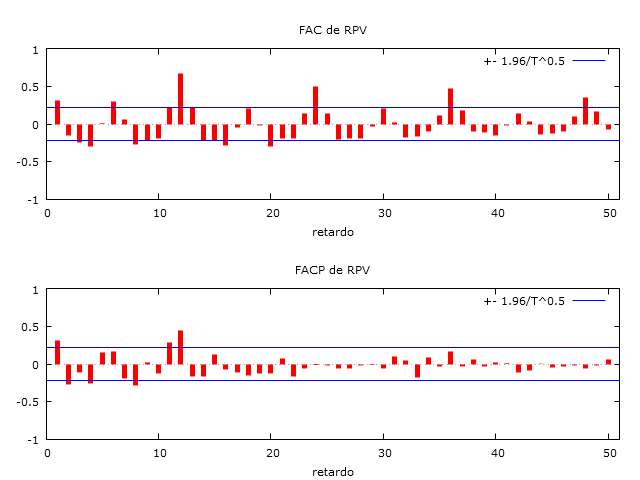
\includegraphics [width=0.8\textwidth]{LOL2}
\label{correlograma1}
\end{figure}

De este correlograma puede observarse que las barritas son la representacion de la correlacion de los retardos y las que no se salen de las lineas horizontales son significativamente iguales a cero y las que no se salen son los retardos con correlacion significativamente diferente de cero.

\textbf{¿Cómo identificar cuando los datos de una serie muestran tendencia?}

Si una serie muestra una tendencia, hay una relación significativa entre los
valores sucesivos de la serie de tiempo. Los coeficientes de autocorrelación son
usualmente grandes para varios de los primeros retrasos de tiempo y luego,
conforme se incrementa el número de retrasos, caen gradualmente hacia cero; 
Una serie de tiempo estacionaria es aquella cuyas propiedades estadísticas
básicas, como la media y la varianza, permanecen constantes en el tiempo,
por lo tanto, se dice que una serie que varía alrededor de un nivel fijo (sin
crecimiento ni decrecimiento) con el paso del tiempo es estacionaria, se dice
también que una serie que contiene una tendencia es no estacionaria, los
coeficientes de autocorrelación de una serie estacionaria decrecen hacia cero
bastante rápidamente, por lo común después del segundo o tercer retraso
de tiempo, por otro lado, las autocorrelaciones muestrales de serie no estacionaria se permanecen muy grandes durante varios periodos.

\textbf{¿Cómo identificar estacionalidad en una serie temporal?}

Si una serie es estacional, un patrón relacionado con el calendario se repite
así mismo durante un intervalo de tiempo específico (generalmente un año).
Las observaciones de la misma posición, en diferentes periodos estacionales,
tienden a estar relacionadas. Si se analizan datos trimestrales que tienen un
patrón estacional, los primeros trimestres tienden a parecerse, los segundos
trimestres tienden a parecerse, y así sucesivamente, y habrá un coeficiente de
autocorrelación significativo en el retraso de tiempo 4, si se analizan datos
mensuales, aparecer´a un coeficiente de autocorrelación significativo en el retraso de tiempo 12, es decir, enero se correlacionará con otros eneros, febrero
se correlacionará con otros febreros y así sucesivamente, un ejemplo de ello se nota en el gráfico \ref{correlograma1} para un retraso de tiempo 12.

\subsection{Metodología Box-Jenkins}

La metodología Box-Jenkins para generar pronósticos es diferente de la
mayoría de los métodos porque no supone ningún patrón particular en los
datos históricos de las series que se van a pronosticar, se basa en un enfoque iterativo para identificar un modelo posible a partir de una clase general
de modelos, luego, el modelo seleccionado se coteja con los datos históricos
para ver si describe la serie con exactitud, el modelo está bien ajustado si
los residuos son generalmente pequeños, están distribuidos aleatoriamente y
no contienen información útil, si el modelo especificado no es satisfactorio,
el proceso se repite usando un nuevo modelo diseñado para mejorar el original, este procedimiento iterativo continúa hasta que se encuentra un modelo
satisfactorio, en ese momento, el modelo se considera útil para pronosticar.
La selección inicial de un modelo ARIMA se basa en examinar una gráfica
de la serie de tiempo (para observar su carácter general) y en analizar sus
autocorrelaciones para varios retrasos de tiempo, específicamente, el patrón
de las autocorrelaciones muestrales calculado a partir de la serie de tiempo
se coteja con el patrón conocido de autocorrelación asociado con un modelo
ARIMA particular, este acoplamiento se hace tanto para las autocorrelaciones como para las autocorrelaciones parciales \cite{Isaac}.

\subsection{Modelo autoregresivos integrados de media movil ARIMA(p,d,q)}

Este modelo es la composicion de un modelo AR(p) y un MA(q) \cite{Cryer} y tambien esta basado en el
supuesto de estacionariedad, esto es, la media y la varianza para una serie de
tiempo son constantes en el tiempo y la covarianza es invariante en el tiempo,
pero se sabe que muchas series de tiempo y en especial las series económicas
no son estacionarias, porque pueden ir cambiando de nivel en el tiempo o
sencillamente la varianza no es constante en el tiempo, a este tipo de proceso
se les considera procesos integrados, por consiguiente, se debe diferenciar
una serie de tiempo "d" veces para hacerla estacionaria y luego aplicarla a esta
serie diferenciada un modelo ARMA(p, q) , se dice que la serie original es
ARIMA(p, d, q)\footnote{Observe que cuando q = 0, el modelo ARMA(p, 0) se reduce a un modelo autorregresivo puro de orden p, de forma similar, cuando p = 0, el modelo ARMA(0, q) es un
modelo de promedio móvil puro de orden q}, es decir, una serie de tiempo autoregresiva integrada de
media m´ovil, donde "p" denota el número de términos autoregresivos, "d" es el
número de veces que la serie debe ser diferenciada para hacerla estacionaria
y "q" el número de términos de la media móvil.

El modelo teórico es el siguiente:

$(1-\phi_1 B - \phi_2 B^2 - ... - \phi_p B^p)(1-B)^d Y_t = (1-  \theta_1 B- \theta_2 B^2-· · ·- \theta_q B^q)\varepsilon_t$

$B^k(Y_t) = Y_{t-k}$ es el operador de retardos o retroactivo.

\subsection{Proceso estacional autoregresivos integrados de media movil SARISMA(P,D,Q)}

Segun \cite{Cryer} cuando una serie de tiempo en estudio tiene intervalos de observación menores a un año, entonces es frecuente que estas tengan variaciones o patrones
sistemáticos cada cierto periodo, estas variaciones sistemáticas inferiores a un
año por ejemplo semestral, mensual, diario, etc., deben ser captadas en los
llamados "Factores Estacionales", dentro de la estructura del modelo a construirse, cada una de estas series puede ser estacionaria o no estacionaria, de
esta manera se combinan términos ordinarios del proceso ARMA y términos
estacionales, así como diferencias regulares y diferencias estacionales para
transformar en series estacionarias; este tipo de procesos
tiene las siguientes características:

\begin{enumerate}

\item Contiene una componente ARIMA(p, d, q) que modela la dependencia regular, que es la dependencia asociada a observaciones consecutivas.

\item Contiene una componente ARIMA(P, D, Q) que modela la dependencia estacional, que está asociada a observaciones separadas por periodos.

\end{enumerate}

El modelo teórico es el siguiente:


$Y_t = c + \overbrace{\phi_1 Y_{t-1}+ ... + \phi_p Y_{t-p}}^{AR(p)}+ \overbrace{\Phi_1 Y_{t-s}+\Phi_2 Y_{t-2s}+...+\Phi_p Y_{t-P_s}}^{SAR(P)} + \\ \underbrace{\varepsilon_t - \theta_1 \varepsilon_{t-1} -...- \theta_q \varepsilon_{t-q}}_{MA(q)} - \underbrace{\Theta_1 \varepsilon_{t-s} - ... - \Theta_q\varepsilon_{t-Q_s}}_{SMA(Q)}$



\subsection{Seleccion, validación del modelo y elaboracion de pronósticos}

\textbf{Selección del modelo}

Para tener una idea del valor de p,q,P y Q para el modelo ARIMA(p,d,q)*(P,D,Q) se hacen uso de las herramietas graficas: Correlogramas, Correlograma extendido, una vez selecionado los valores de p,q,P y Q, se prueban los modelos y se comparan con los criterios de selecion AIC, BIC \cite{Shumway}, cuando ya se ha selecionado el modelo con el menor valor de AIC y BIC entonces se procede a la validación.

\textbf{Validación del modelo}

Para validar el modelo selecionado deben de cumplirse los siguientes supuestos:

\begin{enumerate}
 \item Debe probarse que los residuos del modelo tienen una distribución normal. 
 \item Los resíduos deben tener media 0 y varianza constante (ser ruido blanco).
 \item Las autocorrelaciones residuales individuales deben ser pequeñas y generalmente dentro de         la banda del correlograma y deben ser muy próximas a cero.
 \item Las autocorrelaciones residuales como un grupo deben ser congruentes con aquellas producidas por los errores aleatorios, una verificación
general de la idoneidad del modelo se realiza mediante una prueba de
distribución chi cuadrada $(\emph{X}^2)$ con base en el estadísstico Q de LjungBox\footnote{Si el valor p asociado con el estadístico Q es pequeño (digamos, el valor
p < 0,05), el modelo se considera inadecuado.}

\end{enumerate}

\textbf{Elaboración de pronósticos}

Una vez que se ha encontrado un modelo adecuado, es factible elaborar los pronósticos de uno o varios periodos futuros, con base en los
pronósticos también se pueden construir intervalos de predicción, en
general, para un nivel de confianza dado, cuanto más largo sea el tiempo guía del pronóstico, mayor será el intervalo de predicción, esto es
razonable, puesto que se espera que la incertidumbre sea mayor para
el pronóstico de un valor distante que para el pronóstico de, digamos,
la siguiente observación. El cálculo de los pronósticos e intervalos de
predicción es una labor tediosa y es preferible dejarla a la computadora,
los programas de computadora que ajustan modelos ARIMA generan
pronósticos e intervalos de predicción a requerimiento del analista \cite{Isaac}.




\chapter{Metodología}
\section{Tipo de Investigación}
Se realiza un estudio descriptivo retrospectivo porque es un estudio longitudinal en el tiempo que se analiza en el presente, pero con datos del pasado.
\section{Población}
Se cuenta con una cantidad de registros del consumo energético mensuales de la UES FMOcc desde enero del 2009 hasta agosto de 2015.
\section{Intrumentos}
Con el propósito de obtener un modelo que se ajuste a las series de tiempo
se utilizan softwares para determinar el mejor modelo, éstos son: Gretl, R y
SPSS.

\section{Procedimiento}

Previo a la utilización de la metodología
ARIMA se verifica que las series cumplieran con los requisitos recomendados por algunos autores: consistencia, estabilidad y no existencia de valores
perdidos y que tuvieran un número suficiente de observaciones (más de 50
observaciones por cada serie temporal), la existencia de autocorrelación se
explora mediante el gráfico de las funciones de autocorrelación o correlograma y los ordenes de los términos incluidos en los diferentes modelos se correspondieron con los coeficientes de correlación simple y parcial estadísticamente
significativos, para la selección del modelo adecuado se sigue la metodología
Box-Jenkins que consta de las siguientes etapas :Identificación, Estimación,
Diagnosis o chequeo y Predicciones (Pronósticos), se sigue ésta metodología
siempre que la serie sea estacionaria en media y en varianza, para lograr la
estacionariedad de la serie y estabilizar la media y las autocorrelaciones se
realizan diferenciaciones, es decir reemplazar las observaciones por el valor de
la diferencia entre esta y la observación anterior para la diferenciación regular
(de orden 1) o reemplazarla por la diferencia entre la observación actual y la
correspondiente al periodo estacional anterior para la diferenciación estacional. Además se efectúa, sobre todo transformación de Box-Cox a los datos
para la estabilizacion de la varianza, la busqueda del modelo que mejor se
ajuste a las series se efectúa tratando de que sean sencillos, explicaran bien
las correlaciones internas del proceso y produjeran una diferencia mínima
entre el valor observado y el esperado. Esto se realiza de manera iterativa,
probando las combinaciones más lógicas de términos regulares AR y MA y
de términos estacionales SAR y SMA, incluyendo las diferenciaciones necesarias. La adecuación de un modelo se estableció a partir del análisis de la
significación estadística de los parámetros del mismo, de las características
de los residuos o errores producidos por el modelo sobre la serie y del valor del error de predicción, se utiliza el Porcentaje de Error Medio Absoluto
(MAPE).
\chapter{Analisis de los Datos}
Presentacion de los datos:

\begin{table}[ht]
\caption{Registros del consumo energetico en Kw/h} \label{Datos}
\centering
\begin{tabular}{lrrrrrrr}
\hline
  \hline
  Meses/Años & 2009& 2010& 2011& 2012& 2013& 2014& 2015 \\ 
  \hline
Enero    &6299&	9652&	10921&	8788&	10922&	11786&	11024 \\
    \hline
Febrero    &18237&	20676&	22251&	18085&	20625&	19406&	18593 \\
    \hline
Marzo    &26416&	35408&	36067&	32867&	34239&	33325&	32106 \\
    \hline
Abril    &30059&	31546&	42266&	29160&	30327&	41981&	31394 \\
    \hline
Mayo    &37505&	41199&	29261&	34341&	37033&	29850&	41651 \\
    \hline
Junio    &39370&	42164&	38202&	35712&	38811&	38354&	41560 \\
    \hline
Julio    &35814&	33579&	16255&	29565&	33884&	35204&	35915 \\
    \hline
Agosto    &19151&	27229&	24435&	23470&	27635&	25858&	25756 \\
    \hline
Septiembre    &38658&	40030&	34671&	33122&	41097&38512	& \\
    \hline
Octubre  &38994&	37948&	31354&	35154&	40081&	41093& \\
    \hline
Noviembre  &38993&	38354&	28972&	33985&	39675&	38201& \\
    \hline
Diciembre    &36617&	34544&	30023&	31293&	35763&	34900& \\	

\hline
   \hline
\end{tabular}
\caption*{Fuente: \cite{ANelson}}
\end{table}

La tabla \ref{Datos} muestra la poblacion de registros del consumo electrico de la UES FMOcc desde enero de 2009 hasta agosto de 2015 en Kw/h,\footnote{Kilowatts por Hora} en una primera observación puede notarse como el cosumo para el mes de enero y diciembre varían mucho del resto, es decir, es lógico suponer que en los meses de vacaciones la UES FMOcc consuma menos cantidad de energía.
\newpage
Su representacion gráfica\footnote{Realizada con Gretl} como una serie de tiempo es la siguiete:

\begin{figure}[htb]

\centering
\caption{Serie de tiempo de los datos del consumo enérgetico} 
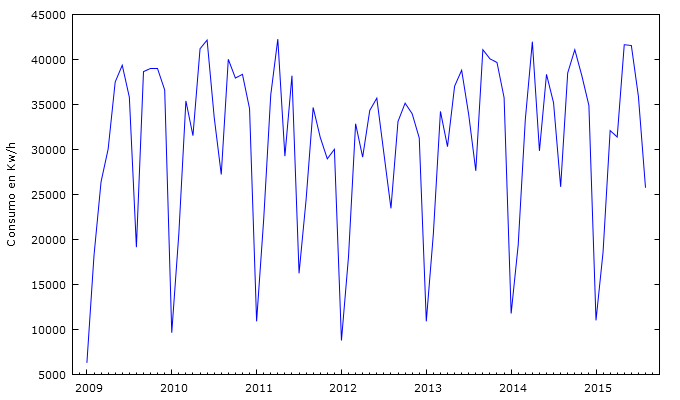
\includegraphics [width=0.8\textwidth]{Graf1}
\caption*{Fuente: Propia} \label{Graf}

\end{figure}

Del gráfico \ref{Graf} puede notarse como el comportamiento del cosumo electrico pareciera ser ciclico o estacional, dado que se repite cada año, en palbras mas sencillas si se trazara una linea vertical en la marca de cada año (sobre el eje horizontal) podria observarse como se forma una especie de "M" en cada año denotando un patron estacional claro, Ademas la serie pareciera sser no estacionaria tanto en media como en varianza, para probar esto se hara uso de la prueba de Dickey Fuller Aumentada realizada con el sofware R.

\begin{Schunk}
\begin{Sinput}
> #cargando librerías necesarias
> library(tseries)
> library(xts)
> library(fUnitRoots)
> #cargando base de datos
> datosSII<-read.csv("SeriesDatosSII.csv", header = TRUE,sep = ",")
> #aplicando formato de serie temporal
> Base<- ts(datosSII$RPV, start = c(2009,1), end = c(2015,8), frequency = 12)
> #Test ADF con constante y tendencia
> ADF1<-adfTest(Base, lags = 11, type = "ct")
> #Test ADF con constante
> ADF2<-adfTest(Base, lags = 11, type = "c")
\end{Sinput}
\end{Schunk}

\begin{table}[ht]
\caption{Test de Dickey Fuller Aumentado} \label{Test1}
\centering
\begin{tabular}{lr}
\hline
  \hline
 \multicolumn{2}{|c|}{$H_0$: existencia de raíz unitaria: a = 1 }\\
 \hline
Tipo de contraste & P-valor\\ 
 \hline
Con constante & 0.7238\\
 \hline
Con constante y tendencia & 0.9414\\

\hline
   \hline
\end{tabular}
\caption*{Fuente: Propia}
\end{table}

De la tabla \ref{Test1} puede concluirse que la serie no es estacionaria ya que el P-valor de la prueba de ADF es mayor a 0.05 por lo que hay existencia de raiz unitaria y por lo tanto la serie es no estacionaria.

\begin{figure}[htb]

\centering
\caption{Correlogramas FAC y FACP de los datos del consumo enérgetico} 
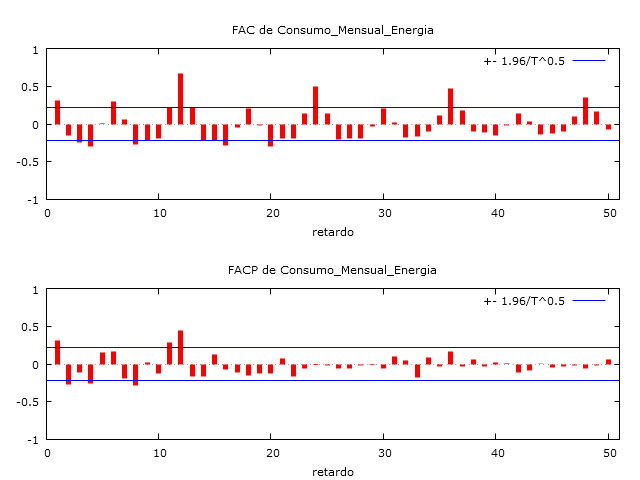
\includegraphics [width=0.8\textwidth]{CX}
\caption*{Fuente: Propia} \label{Graf2}

\end{figure}

El gráfico \ref{Graf2} desarrollado en Gretl, muestra tambien como la serie es no estacionaria dado que varios de los primeros retardos en FAC y FACP son significativamente diferentes de cero ademas puede notarse que los retardos 1, 12, 24, 36 y 48 para FAC poseen una correlacion significativamente diferente de cero lo que da la pauta para concluir que la serie analizada es estacional.

\section{Estacionarización de los datos}

Para estacionarizar los datos se hará uso de una diferencia estacional para estabilizar en media y reducir la estacionalidad y de la transformación de box-cox para estabilizar la varianza, este analisis se desarrollará en R.

\begin{Schunk}
\begin{Sinput}
> #cargando librerías necesarias
> library(tseries)
> library(xts)
> library(TSA)
> #cargando base de datos
> datosSII<-read.csv("SeriesDatosSII.csv", header = TRUE,sep = ",")
> #aplicando formato de serie temporal
> Base<- ts(datosSII$RPV, start = c(2009,1), end = c(2015,8), frequency = 12)
> #buscando un lambda para la transdormació
> BoxCox.ar(datosSII$RPV)
> #Aplicando la diferecia estacional
> #con el retardo 12
> DFE<-diff(Base, lag = 12)
\end{Sinput}
\end{Schunk}

\begin{figure}[htb]

\centering
\caption{Test de Box-Cox para encontrar un Lambda Adecuado} 
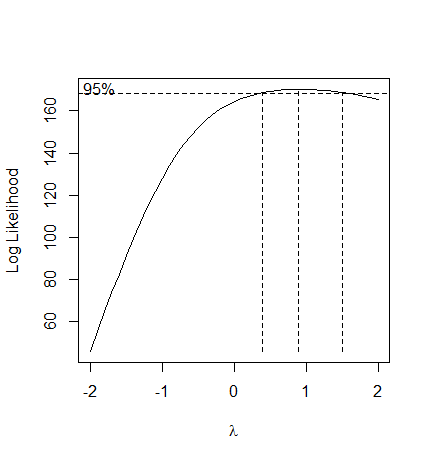
\includegraphics [width=0.4\textwidth]{BoxcoxPlot}
\caption*{Fuente: Propia} \label{Graf3}

\end{figure}
\newpage
Puede observarse en el gráfico \ref{Graf3} que la linea central de las tres lineas verticales punteadas estan cercanas a el valor de 1 por lo que la transformación de Boxcox sugiere que lambda sea igual a 1 con un 95\% de confianza, sin embargo que lambda sea igual a 1 indica que no es necesario aplicar una transformación a los datos.

\begin{figure}[htb]

\centering
\caption{Serie estabilizada en media por una diferecia estacional} 
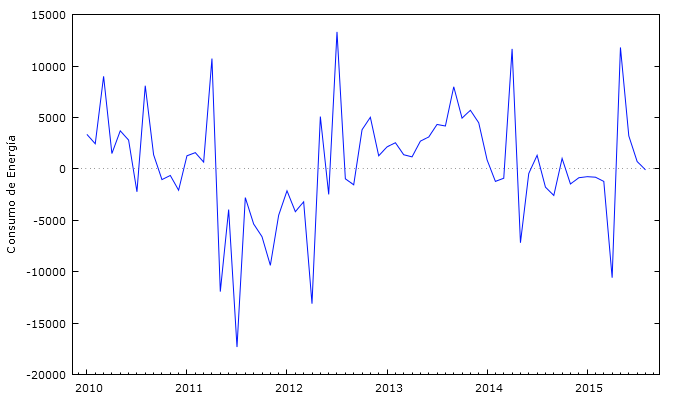
\includegraphics [width=0.5\textwidth]{SerieDIFF}
\caption*{Fuente: Propia} \label{Graf4}

\end{figure}

Del gráfico \ref{Graf4} puede observarse que la serie ha sido estabilizada en media y pareciera que también esta estabilizada en varianza aun sin hacer alguna transformación, sin embargo se realizará el Test de ADF para probar si la serie difereciada es estacionaria.

\begin{table}[ht]
\caption{Test de Dickey Fuller Aumentado} \label{Test2}
\centering
\begin{tabular}{lr}
\hline
  \hline
 \multicolumn{2}{|c|}{$H_0$: existencia de raíz unitaria: a = 1 }\\
 \hline
Tipo de contraste & P-valor\\ 
 \hline
Con constante & 0.00339\\
 \hline
Con constante y tendencia & 0.01873\\

\hline
   \hline
\end{tabular}
\caption*{Fuente: Propia}
\end{table}

Puede observarse que segun la tabla \ref{Test2} el P-valor de la prueba ADF desarrollada en Gretl es menor que 0.05 por lo que hay evidencia estadistica pra rechazar $H_0$ por lo tanto la nueva serie es estacionaria con una diferencia estacional.

\section{Selección del modelo}

El modelo a utilizar sera un SARISMA para ecoger el valor de los retardo se hara uso de los correlogramas de la serie estacionarizada.

\begin{figure}[htb]

\centering
\caption{Correlograma de la serie estacionaria} 
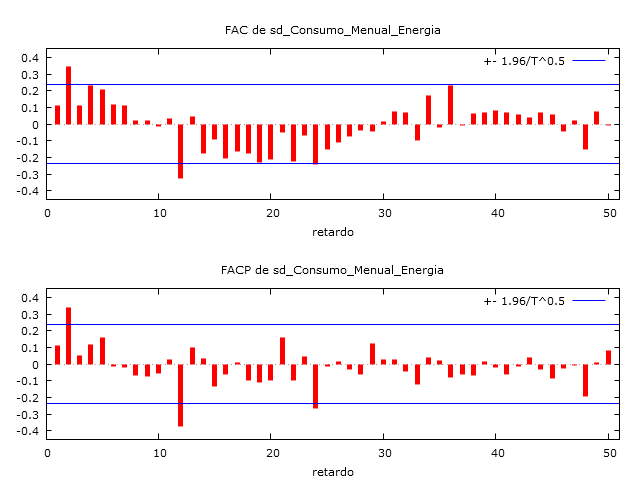
\includegraphics [width=0.5\textwidth]{CEST}
\caption*{Fuente: Propia} \label{Graf5}

\end{figure}

Puede observarse en el gráfico \ref{Graf5} que para la FAC el segundo retardo es considerablemente diferente de cero por lo que sugiere un modelo ARIMA(0,0,2) y con su componente estacional SARISMA(0,1,1)\footnote{En este caso D=1 por que fue difereciada estacionalmente una sola vez.}, al mismo tiempo el correlograma segun el FACP sugiere ARIMA(2,0,0) dado que el retardo 2 es considerablemente diferente de cero y su componente estacional un SARISMA(1,1,0), Entonces tenemos dos posibilidades un SARISMA(2,0,0)*(1,1,0) ó un SARISMA(0,0,2)*(0,1,1). se hara el ajuste de ambos modelos y se escogera el que sea mas significativo estadisticamente.

\subsection{Ajuste del modelo SARISMA(2,0,0)*(1,1,0)\\ y SARISMA(0,0,2)*(0,1,1)}

Al hacer el ajuste en Gretl pudo observarse lo siguiente:

\textbf{Ajuste del modelo SARISMA(2,0,0)*(1,1,0)}

\begin{center}
\begin{table}[htb]
\caption{Estadísticos de comparación}
\begin{tabular}{lrlr}
 \hline
Media de la vble. dep. &  361.6471 & D.T. de la vble. dep. &  5589.167 \\
 \hline
media innovaciones &  39.44258 & D.T. innovaciones &  4746.117 \\
 \hline
Log-verosimilitud & $-$673.2666 & Criterio de Akaike &  1356.533 \\
 \hline
Criterio de Schwarz &  1367.631 & Hannan--Quinn &  1360.930 \\
 \hline
\end{tabular}
\caption*{Fuente: Propia} \label{xDD}
\end{table}
\end{center}

Puede observarse en la tabla \ref{xDD} que el AIC, y el HQC tienen un valor de 1356.533 y 1360.930
respectivamente lo que servira de comparacion para el siguiente modelo.


\textbf{Ajuste del modelo SARISMA(0,0,2)*(0,1,1)}

\begin{center}

\begin{table}[htb]
\caption{Estadísticos de comparación}
\begin{tabular}{lrlr}
 \hline
Media de la vble. dep. &  361.6471 & D.T. de la vble. dep. &  5589.167 \\
 \hline
media innovaciones & $-$153.5331 & D.T. innovaciones &  3649.986 \\
 \hline
Log-verosimilitud & $-$665.7208 & Criterio de Akaike &  1341.442 \\
 \hline
Criterio de Schwarz &  1352.539 & Hannan--Quinn &  1345.839 \\
 \hline
\end{tabular}
\caption*{Fuente: Propia} \label{xDD2}
\end{table}

\end{center}

Puede observarse en la tabla \ref{xDD} que el AIC, y el HQC tienen un valor de 1341.533 y 1345.930
respectivamente lo que servira de comparacion para escoger el modelo.

\textbf{Conclusíon}

Dado que el AIC y el HQC son mas pequeños en el ajuste del modelo SARISMA(0,0,2)*(0,1,1) se selecionara éste para el analisis de los datos del consumo de energía.

\section{Validación del modelo}

En esta etapa se comprueba la normalidad de los resíduos del modelo y
la incorrelación de los resíduos, si una de estas condiciones no se cumple es
porque el modelo no es adecuado.

\subsection{Incorrelación en los residuos}

\begin{figure}[htb]

\centering
\caption{Correlograma de la serie estacionaria} 
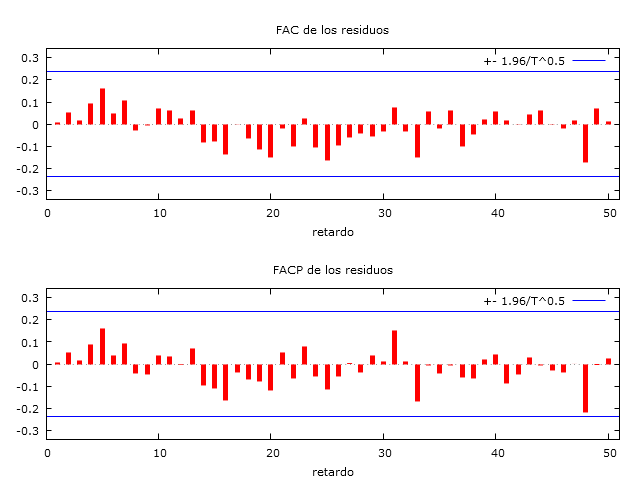
\includegraphics [width=0.5\textwidth]{Modelo}
\caption*{Fuente: Propia} \label{Graf6}

\end{figure}

El gráfico \ref{Graf6} muestra que los resíduos del modelo SARISMA identificado
son incorrelados, es decir, todos o la mayoría no se salen de las bandas rojas que representan el intervalo de confianza a un nivel de confianza el 95
por ciento.

\subsection{Normalidad en los residuos}

\begin{figure}[htb]

\centering
\caption{Correlograma de la serie estacionaria} 
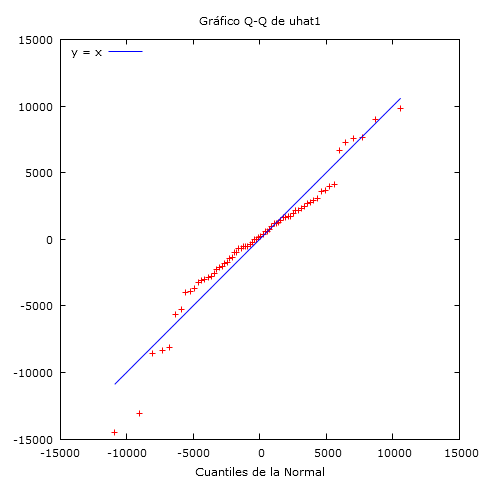
\includegraphics [width=0.5\textwidth]{ModeloQQ}
\caption*{Fuente: Propia} \label{Graf7}

\end{figure}

Para verificar la normalidad de los residuos se utiliza el estadístico Chi
cuadrado con hipótesis nula: Existe normalidad, y el gráfico QQ (\ref{Graf7}) de los
resíduos  el cual comprueba la existencia de normalidad si los puntos del
gráfico de dispersión se ajustan muy bien a la recta con pendiente positiva y = x. El p valor de la prueba es igual a
0,8828, como el p valor es mayor que el nivel de significancia de cinco por
ciento entonces se acepta la hipótesis nula de que los resíduos del modelo son
normales.

\section{Proyecciones}


\begin{figure}[htb]

\centering
\caption{Correlograma de la serie estacionaria} 
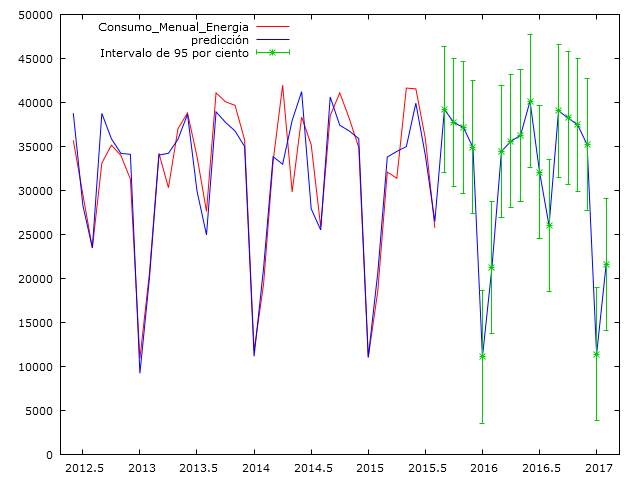
\includegraphics [width=0.5\textwidth]{Proyecciones}
\caption*{Fuente: Propia} \label{Graf8}

\end{figure}

\begin{center}
 Para intervalos de confianza 95\%, $z(0.025) = 1.96$

\end{center}

\begin{center}
\begin{table}[htb]
\caption{Proyecciones del Modelo}
\begin{longtable}{%
r% col 1: obs
  r@{.}l% col 2: actual
    r@{.}l% col 3: fitted
      r@{.}l% col 4: std error
        r@{.}l% col 5: conf int lo
         r@{.}l}% col 5: conf int hi
Observaciones & \multicolumn{2}{c}{Consumo\_Mensual\_Energia}  & \multicolumn{2}{c}{predicción}
  & \multicolumn{2}{c}{Desv. Típica}
   & \multicolumn{4}{c}{Intervalo de 95\% } \\[1ex]
     \hline
 2015:09  & \multicolumn{2}{c}{} & 39211&16 & 3649&986 & 32057&32 & 46365&00 \\
  \hline
 2015:10  & \multicolumn{2}{c}{} & 37730&96 & 3689&022 & 30500&61 & 44961&31 \\
  \hline
 2015:11  & \multicolumn{2}{c}{} & 37162&87 & 3842&656 & 29631&40 & 44694&34 \\
  \hline
 2015:12  & \multicolumn{2}{c}{} & 34917&81 & 3842&656 & 27386&34 & 42449&28 \\
  \hline
 2016:01  & \multicolumn{2}{c}{} & 11111&38 & 3842&656 & 3579&91 & 18642&85 \\
  \hline
 2016:02  & \multicolumn{2}{c}{} & 21278&06 & 3842&656 & 13746&59 & 28809&52 \\
  \hline
 2016:03  & \multicolumn{2}{c}{} & 34445&35 & 3842&656 & 26913&88 & 41976&82 \\
  \hline
 2016:04  & \multicolumn{2}{c}{} & 35614&87 & 3842&656 & 28083&40 & 43146&34 \\
  \hline
 2016:05  & \multicolumn{2}{c}{} & 36255&81 & 3842&656 & 28724&35 & 43787&28 \\
  \hline
 2016:06  & \multicolumn{2}{c}{} & 40159&68 & 3842&656 & 32628&21 & 47691&15 \\
  \hline
 2016:07  & \multicolumn{2}{c}{} & 32107&43 & 3842&656 & 24575&96 & 39638&89 \\
  \hline
 2016:08  & \multicolumn{2}{c}{} & 26020&34 & 3842&656 & 18488&87 & 33551&80 \\
  \hline
 2016:09  & \multicolumn{2}{c}{} & 39060&78 & 3842&656 & 31529&31 & 46592&25 \\
  \hline
 2016:10  & \multicolumn{2}{c}{} & 38251&39 & 3842&656 & 30719&92 & 45782&86 \\
  \hline
 2016:11  & \multicolumn{2}{c}{} & 37471&91 & 3842&656 & 29940&44 & 45003&38 \\
  \hline
 2016:12  & \multicolumn{2}{c}{} & 35226&85 & 3842&656 & 27695&38 & 42758&32 \\
  \hline
 2017:01  & \multicolumn{2}{c}{} & 11420&42 & 3842&656 & 3888&95 & 18951&89 \\
  \hline
 2017:02  & \multicolumn{2}{c}{} & 21587&10 & 3842&656 & 14055&63 & 29118&56 \\
  \hline
\end{longtable}
\caption*{Fuente: Propia}\label{xDDD}
\end{table}
\end{center}



Puede observarse en el gráfico \ref{Graf8} las proyeciones realizadas por el modelo y como éste se ajusta considerablemente bien a los datos originales, ademas en la tabla \ref{xDDD} puen observarse las proyeciones de energía que sera consumida en los proximos 18 meses junto con sus intervalos de confianza.


\chapter*{Conclusiones}
\addcontentsline{toc}{chapter}{Conclusiones}
En Respuesta a las Hipotesis y preguntas de Investigación:
\begin{enumerate}
  \item Para la Hipotesis 1. No hay suficiente evidencia para rechazar la hipotesis nula por lo que se concluye que NO hay eficiencia enérgetica en los edificios de la UES FMOcc.
  \item Para la Hipotesis 2. Hay suficiente evidencia para rechazar la Hipotesis nula por lo que dada las proyecciones realizadas pudo determinarse que el consumo energetico es estable a través del tiempo, sin embargo puede llegar a reducirse.
  \item Para la Hipotesis 3. No hay suficiente evidencia para rechazar la hipotesis nula por lo que se concluye que el periodo de tiempo donde mas energía se consume es el los ciclos activos en la UES FMOcc.
  \item Si es posible alcanzar la eficiencia energetica a través de las propuestas de \cite{ANelson} que sugieren la reduccion del consumo energetico y su costo.
  \item La cantidad de energía Ahorrada dependera de la correcta aplicacion de las propuestas de \cite{ANelson} y podria llegar a ahorrase hasta un 30\%- 60\% en un largo plazo de 18 meses.
\end{enumerate}

En respuesta a los Objetivos:

\begin{enumerate}
  \item Si se logro desarrollar las proyecciones del consumo energetico a través de una serie temporal
  \item El periodo de tiempo donde se consume mayor cantidad de energía según los datos y las proyeciones analizadas es en los meses de Febrero, Marzo, Abril, Mayo, Junio, Septiembre, Octubre, Noviembre y donde es mas bajo el consumo en Enero, Julio, Agosto y Diciembre.
  \item Este objetivo sera respondido gracias al trabajo de \cite{ANelson} de la siguiente manera.
\end{enumerate}

\section*{Medidas Correctivas}

\addcontentsline{toc}{chapter}{Medidas Correctivas}

Algunas de las medidas consideradas en este trabajo gracias a \cite{ANelson} son las siguientes:

\textbf{Problema 1.}

\textbf{Descripción:}

El sistema de climatización de la Facultad Multidisciplinaria de Occidente consta de demasiadas unidades de aire acondicionado con baja capacidad de refrigeración (capacidad máxima de 5 Toneladas de Refrigeración (TR)), esto causa el inconveniente que deban emplazarse muchas unidades para satisfacer la demanda térmica de un edificio, como el caso del edificio de Carreras Múltiples donde hay 20 aires acondicionados emplazados para una capacidad instalada de 75 TR, donde pudo emplazarse tres unidades de 25 TR. El problema es el consumo de energía eléctrica excesivo en 20 aires acondicionados comparado con el consumo de tres o cuatro unidades que sumen la misma capacidad de 75 TR; entonces, cuando se tenga que sustituir el sistema de climatización debe evaluarse la alternativa de emplazar una sola unidad que suministre la demanda térmica completa del edificio y que proporcione menor consumo de energía.
Además se aumentan los costos de mantenimiento, ya que, se tiene que intervenir correctiva y preventivamente a las 20 unidades realizando sustitución de piezas y partes como condensadores, compresores, también recargar el fluido refrigerante, revisar sistema eléctrico, entre otras intervenciones a varias de las unidades al mismo tiempo, en cambio si se tiene solo una unidad exterior de aire acondicionado el mantenimiento preventivo y correctivo será exclusivo para ésta ahorrando incluso recurso humano.
El tener una sola unidad exterior no quiere decir, que si se encuentra está en funcionamiento, todas las oficinas estarán climatizadas aunque estén vacías, ya que, este tipo de aires acondicionados de gran capacidad permiten instalar varias unidades interiores cada una de las cuales se controla individualmente permitiendo tener oficinas con el aire acondicionado apagado, incluso oficinas a diferentes temperaturas.

\textbf{Medida correctiva}

Consiste en sustituir los aires acondicionados de baja capacidad de refrigeración instalados en los edificios por una unidad climatizadora individual que cubra la misma demanda térmica que los equipos sustituidos. La acción está pensada primeramente para disminuir el consumo de electricidad que provoca el tener demasiadas unidades de aire acondicionados instaladas; la nueva unidad climatizadora además de proporcionar la misma capacidad de refrigeración tiene un consumo menor de electricidad como consecuencia principal de que solo se tendrá un compresor demandando potencia de funcionamiento a diferencia de tener 20 compresores demandando potencia en el caso los 20 aires acondicionados del edificio de Carreras Múltiples. Además se mejorará la gestión del mantenimiento de este sistema.

\textbf{Problema 2.}

\textbf{Descripción.}

Las oficinas y laboratorios que cuentan con aire acondicionado instalado no tienen sistema de renovación de aire que produce el inconveniente de disminuir la calidad de éste, la causa principal es la concentración de di-óxido de carbono que aumenta progresivamente debido a la transpiración de las personas que se encuentran dentro de la oficina. Instalar un sistema de renovación de aire representa un aumento en la demanda térmica del sistema de climatización, con el correspondiente aumento del consumo en electricidad, sin embargo, es mucho menor que la carga por transmisión, por equipo, por personas y por radiación, pero, lo importante es garantizar la salubridad del aire que las personas respiran cuando se encuentran dentro de las oficinas.

El aire debe de renovarse por lo menos cada hora, sin embargo, el sistema de renovación de aire renovará el aire por lo menos cada hora mientras el aire acondicionado esté en funcionamiento.

Los inconvenientes que causa el no contar con sistema de renovación de aire en las oficinas y laboratorios son los siguientes:

\begin{itemize}

 \item Disminución de la calidad del aire debido por las concentraciones de di-óxido de carbono.
	 \item Aumento de la probabilidad de enfermedades producto de aire contaminado.

\end{itemize}

El no contar con sistema de renovación de aire tiene beneficios desde el punto de vista del consumo como los siguientes:

\begin{itemize}

  \item Disminución de la demanda térmica de las oficinas y laboratorios
  \item Disminución de los costos de la factura eléctrica que se paga a la empresa distribuidora

\end{itemize}

Esta disminución es pequeña, además, no se puede disminuir el consumo de electricidad a costa de la salud y seguridad de las personas y por eso el sistema de renovación de aire es necesario.

\textbf{Medida correctiva}

Consiste en instalar dos ventiladores en la oficina o laboratorio, un primer ventilador que extraiga el aire contaminado del interior del espacio climatizado y un segundo ventilador que introduzca aire salubre del exterior al interior de la oficina. Los sistemas industriales se instalan en el techo de los edificios, sin embargo, el edificio debe contar con un sistemas de ductos de ventilación que conduzcan el aire renovado y contaminado que actualmente no se tiene, esto con el motivo de renovar el aire de todas las oficinas y laboratorios con un solo sistema. También se puede instalar un sistema individual en cada oficina o laboratorio simplemente con dos ventiladores pequeños.
Hay lugares donde no es estrictamente necesario el sistema de renovación de aire, en especial aquellos donde se concentran menos de cinco personas; una solución práctica sería que estas personas tuvieran la responsabilidad de renovar el aire abriendo las ventanas cuando se da el descanso por motivo de almuerzo de 12:00 a 2:00 pm, cerrándolas al terminar el descanso, sería un hábito que mejoraría las condiciones de salubridad del aire. Ahora, los lugares donde es necesario instalar el sistema de renovación son los que tiene altas concentraciones de personas, como salas de exposiciones y conferencias, centros de cómputo, laboratorios  y salones de clase. Entonces en estos se instalará el sistema.

\textbf{Problema 3.}

\textbf{Descripción}

Según la investigación realizada en la Facultad se percibe que uno de las problemáticas más comunes que se presentan, es la falta de sectorización de algunos de los circuitos de luminarias internas de edificios tanto de oficinas administrativas como de áreas comunes como aulas, y con esto se tiene una fuga de energía eléctrica desperdiciada cada vez que son utilizadas las luminarias.

\textbf{Medida Correctiva}

La sectorización por áreas y zonas, es la acción correctiva consiste en realizar el ordenamiento en los circuitos de las luminarias internas que presentan un patrón que no está bien definido o que presentan características que no van de acuerdo al tipo de actividad de se realiza en el lugar. Se presentan dos de los patrones que deberán ser usados en los espacios de donde a color rojo se tienen las secciones de los circuitos como deben ser controlados por un mismo apagador y con esto iluminar zonas independientes de otras.

Patrón 01: Para este corresponde la figura  donde el patrón de los circuitos esta dado como bloques paralelos a la pizarra, donde este está enfocado a aquellas aulas que presentan un nivel de iluminación aproximadamente igual en todos sus puntos y que la iluminación natural no provoca mayor incidencia en los niveles de iluminación del área.

Patrón 02: En este caso la sectorización está dada por con un patrón mixto donde se tienen bloques paralelos a la pizarra de los circuitos controlados por apagadores independientes, pero sumado a esto se tiene una sección que es paralela a las ventanas del aula en cuestión donde puede verse en la figura. Este patrón de conexión de los circuitos de las luminarias es con el fin aprovechar la luz natural proveniente de las ventanas.

Patrón 03: Se propone un tercer caso en donde a criterio de las condiciones que se presentan en el áreas deber ser establecido el orden de los circuitos como es el caso de laboratorios y oficinas, pues en función de las exigencias que se necesitan lumínicamente, así deberá ordenarse donde no hay un patrón establecido.

\textbf{Problema 4.}

\textbf{Descripción }

Se pueden plantear acciones de eficiencia energética bien estructuradas en innovación tecnológica (equipo electrónico de menor consumo), domótica (control automatizado de equipos electrónicos), entre muchas otras que pretendan disminuir el consumo de energía sin tomar en cuenta las práctica humanas; y aun así, tener desperdicio de electricidad debido a las actividades de los seres humanos que favorecen el uso ineficiente de la energía. El problema es, que la comunidad universitaria ejecuta prácticas y tiene hábitos en el uso de equipo eléctrico-electrónico que incurren en desperdicio de energía, se citan unos ejemplos:

\begin{itemize}
\item No apagar iluminación en salones de clase vacíos y áreas de trabajo.
\item Ajustar aires acondicionados con temperaturas diferentes de la temperatura de confort.
\item Comprar equipos electrónicos baratos y de alto consumo eléctrico.
\item Pintar ventanas y colocar cortinas que obstaculizan la luz natural y obligan a utilizar luz artificial.
\end{itemize}

En algunas prácticas es conocido por la mayoría que son causantes de desperdicio energético como: luminarias encendidas y sin uso en salones de clase vacíos; y en otras prácticas no es conocido por la comunidad universitaria que causan desperdicio de energía, como: comprar equipo electrónico barato y de alto consumo de electricidad, ya que, se demuestra con un análisis de costos de todo el ciclo de vida (este suma el precio inicial más los costos de consumo eléctrico durante toda la vida útil del producto) que comprando productos con eficiencia energética alta aunque el precio inicial sea mayor se termina pagando mucho menos en el largo plazo que comprando un producto barato e ineficiente, como en el caso de la luminaria LED.

\textbf{Medida correctiva}

La implementación de Cultura Energética en la UES-FMOcc tiene el objetivo de cambiar la forma de actividad humana en la universidad que favorece el desperdicio de electricidad, por otro tipo de actividad que utilice la electricidad de manera eficiente. Entonces se pretende un cambio en la cultura organizacional, algo muy difícil de lograr y que requiere el apoyo de toda la comunidad tanto en liderazgos formales como informales. La acción correctiva se enfoca a un cambio de hábitos, practicas, costumbres, información, conocimiento y mucho más que favorece el desperdicio de energía, y una de las formas de lograr el cambio es generando conciencia en función de costos-beneficios obtenidos. Utilizando el sentido estricto de la palabra “CONCIENCIA” es lo que se hace, a través de la ciencia (investigación científica) se demuestra que los costos, que su la mayoría no son económicos, sino, de voluntad de la comunidad son mucho menores que los beneficios o dicho de otra forma, el ahorro de energía  trae beneficios de magnitud exponencial que no son solo beneficios económicos sino medio-ambientales.

\textbf{Estas medidas suponen la reducción del consumo energético a corto, mediano y largo plazo, logrando de esta manera obtener un sistema de energía más eficiente.}

\cleardoublepage
\addcontentsline{toc}{chapter}{Bibliografía}
\nocite{*}
\bibliographystyle{apalike}
\bibliography{SIIB}

\end{document}





